\documentclass[]{article}
\usepackage{natbib}
\bibliographystyle{unsrtnat}
\usepackage{graphicx}
%\usepackage{placeins}
\usepackage[british]{babel}
\usepackage[autostyle]{csquotes}
\usepackage{url}
\DeclareGraphicsExtensions{.pdf,.png,.jpeg,.jpg}
\graphicspath{{images/}}
%\graphicspath{ {./images/} }
\usepackage{wrapfig}
\renewcommand{\figurename}{Fig.}
%opening

\title{Identifying macro-moths with micro-features}
\author{Paul J. Palmer}

\begin{document}

\maketitle

\begin{abstract}

This article explores the use of external microscopic features to support the identification (ID) of  macro-lepidoptera. The usual process of identifying macro-moths  focusses on the wings, which are often large and distinctively patterned. Matching an unknown specimen to reference pictures is often the identification method employed, but as shown in the example here, can give a misleading result.
 However, microscopic features may be used to narrow the field of candidate taxa to arrive at a robust identification. 

\end{abstract}

\section*{A Difficult Specimen to ID}
The specimen in question was taken at sugar 2020-08-16 on the Rutland Water Nature Reserve. It would have been recorded as a very worn example of \textit{Hypena proboscidalis} (The Snout) if it had not briefly raised its wings in a posture uncharacteristic for this species, placing an element of doubt in this presumption. As can be seen in Figure~\ref{fig:202009131026pjp-1}, the specimen lacks the long, forward pointing palps that give the Snout its vernacular name, buts its wings have the same slightly hooked shape  and similar median fascia as the verified specimen illustrated in  Figure~\ref{fig:S202012271446-1}.  It would be easy to presume that the palps have been broken in what appears to be a worn specimen, but examination under magnification, as shown in  Figure~\ref{fig:20201112-1} reveals that the palps are short and undamaged. Less obvious, because it is less often mentioned in the descriptive text of guide books, is the lack of ocelli above the compound eye,  which  eliminates \textit{Hypena proboscidalis} as a candidate taxon for the specimen.

\section*{The Identification Method}
Identification of an unknown Lepidoptera specimen may be thought of as the process by which the  observable features are matched to those of a known taxon.
For a general discussion on the topic of identification \citet{Pankhurst1978} is still relevant to the field naturalist today.
 Given that there are about 2,500 UK Lepidoptera taxa of which around 450 are thought of as \enquote{the larger moths} a systematic approach is needed to avoid randomly flipping through the pages of a guide.
 Inspired by Pankhurst, the approach followed by the author is to list candidate species and to mark them with \enquote{+} for matching features and \enquote{-} contradicting features. A \enquote{?} is used to  indicates that a feature is either. \enquote{not known} or not yet determined. An identification is achieved when one of the candidates has multiple \enquote{+} and no \enquote{-} against its name.
 A well written dichotomous key will lead you through a functionally identical process, as will a computer driven \enquote{multi-access} key.
 The take-away message is that a robust identification always relies on the matching and rejection of multiple features, some of which may be hard to see.  
 
 Putting this into practice,  examination of specimens under  3 --- 30 x magnification reveals additional features that should be visible in both live and preserved specimens. The low magnification required places these features in range of hand lenses and USB microscopes. 

\section*{Making a Determination}
We start by noting observation about the unknown specimen:
Forewing length: 16.7 mm; Forewing width: 11.4, mm;  Ocelli: Absent;  Labial palps: Forward. Flight time: August. Gender: Female.

Unfortunately there a few resources listing the features to consider, but a good place to start is the matrix key published by \citet{Dombroskie2011}. While it is intended for Canadian Lepidoptera, it can also be used to provide an indicative guide to UK lepidoptera families. Importantly, it is a useful indication of  features that can be used to find the likely family of a specimen.

%In this case, although the specimen is a macro-moth, the family \textit{Erebidae}.
Using the Canadian Lepidoptera Key , (See Figure~\ref{fig:20201112-1}), the lack of oceli (simple eyes), coiled unscaled proboscis, and forward facing palps are suggestive of family \textit{Geometridae}. The forewing length of 16.7 mm and the flight time of August are also useful for eliminating many possible UK taxa.

A list of candidate \textit{Geometridae} based on size and general appearance can be made using  \citet{Skinner1984} or other guide and is plausibly a single taxon: \textit{Scotopteryx chenopodiata} (Shaded Broad-Bar) , but the specimen appearance is very plain for this species.

The dissection in Figure\ref{fig:202009131026pjp-3}  confirms \textit{Scotopteryx chenopodiata} 

\begin{figure}
	\centering
	\begin{minipage}{0.45\textwidth}
		\centering
	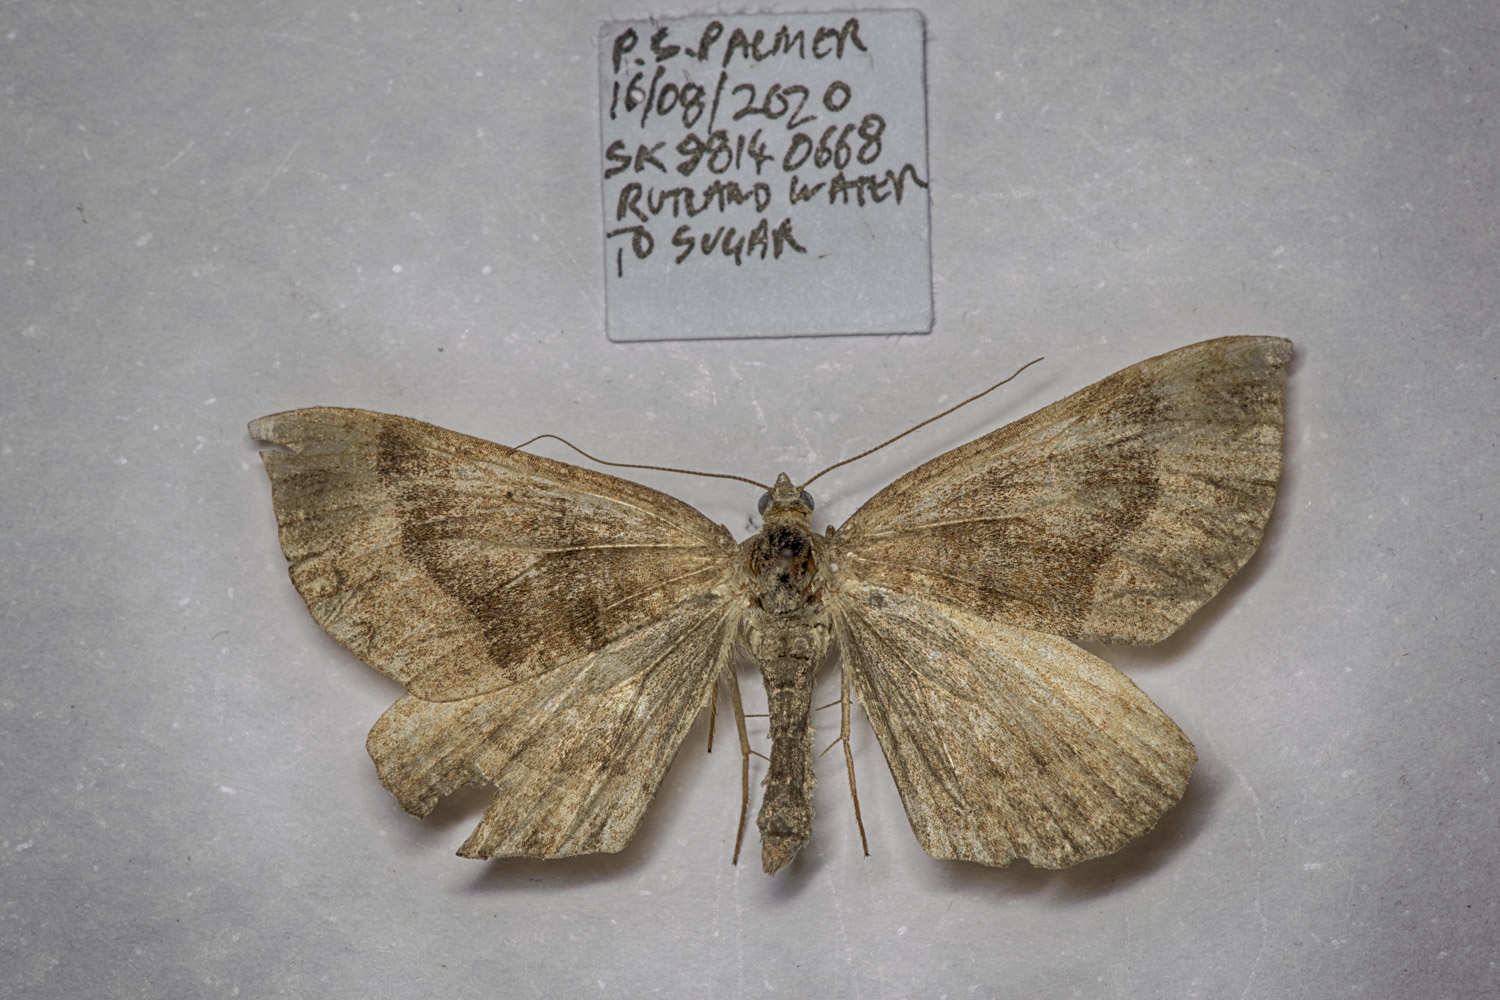
\includegraphics[width=0.9\linewidth]{202009131026PJP-1}
	\caption{The unkown specimen resembling Hypena proboscidalis.}
	\label{fig:202009131026pjp-1}
	\end{minipage}\hfill
	\begin{minipage}{0.45\textwidth}
		\centering
		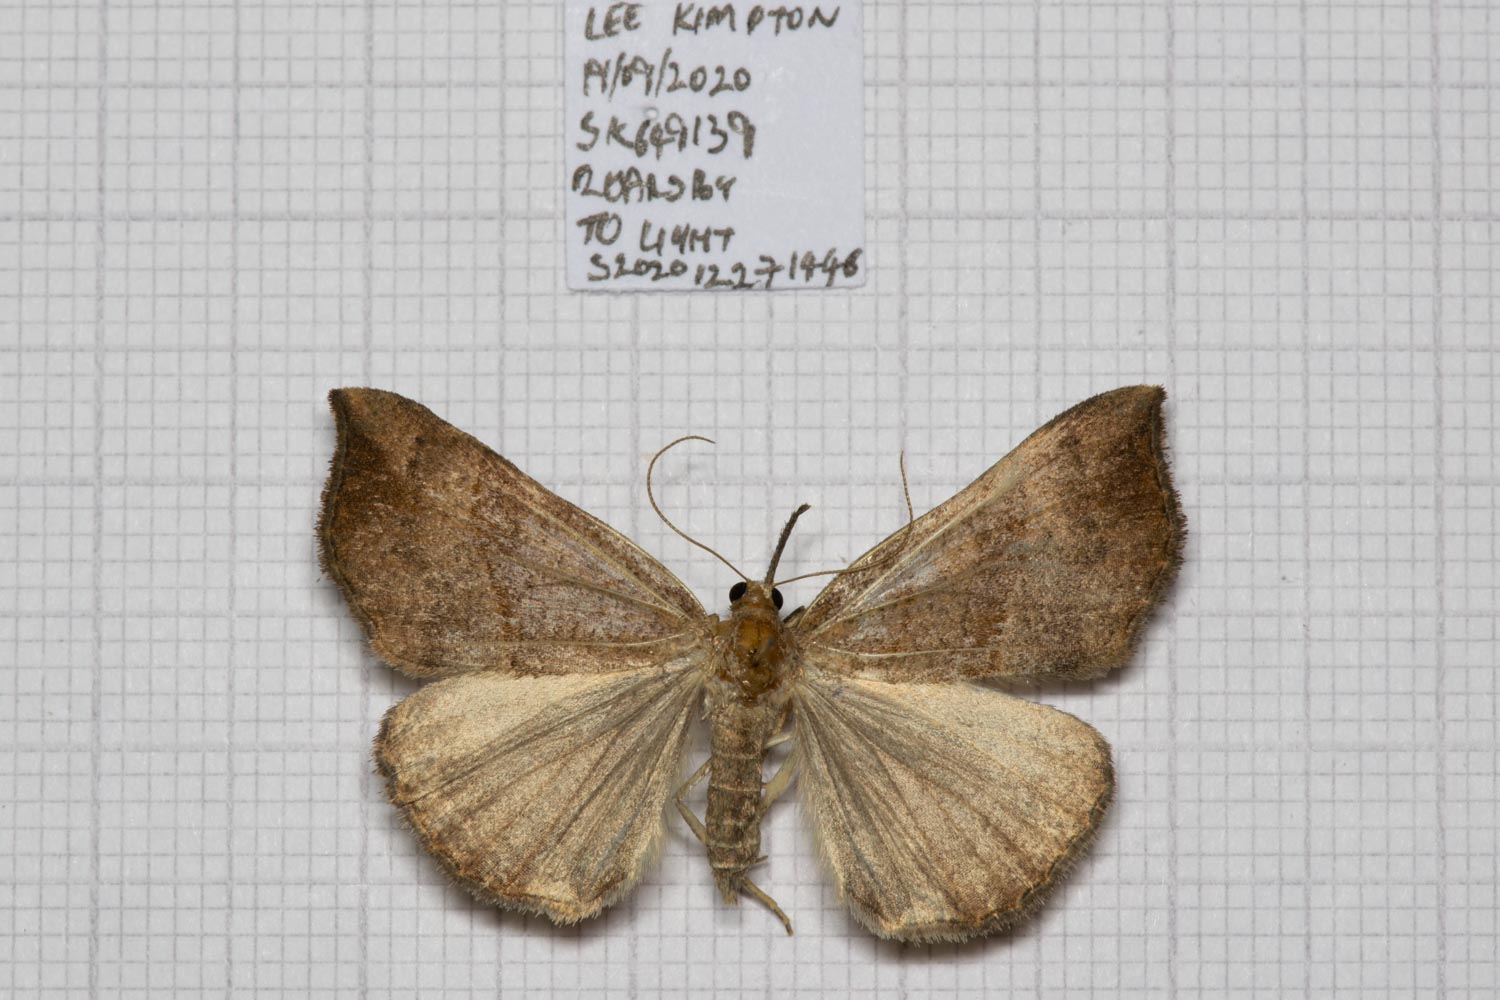
\includegraphics[width=0.9\textwidth]{S202012271446-1} % second figure itself
		\caption{A verified specimen of female Hypena proboscidalis.}
		\label{fig:S202012271446-1}
	\end{minipage}
\end{figure}



\begin{figure}
	\centering
	\begin{minipage}{0.45\textwidth}
		\centering
	\includegraphics[width=0.5\linewidth]{20201112-1}
	\caption{Short undamaged palps eliminate Hypena proboscidalis as a candidate taxon.}
	\label{fig:20201112-1}
	\end{minipage}\hfill
	\begin{minipage}{0.45\textwidth}
		\centering
		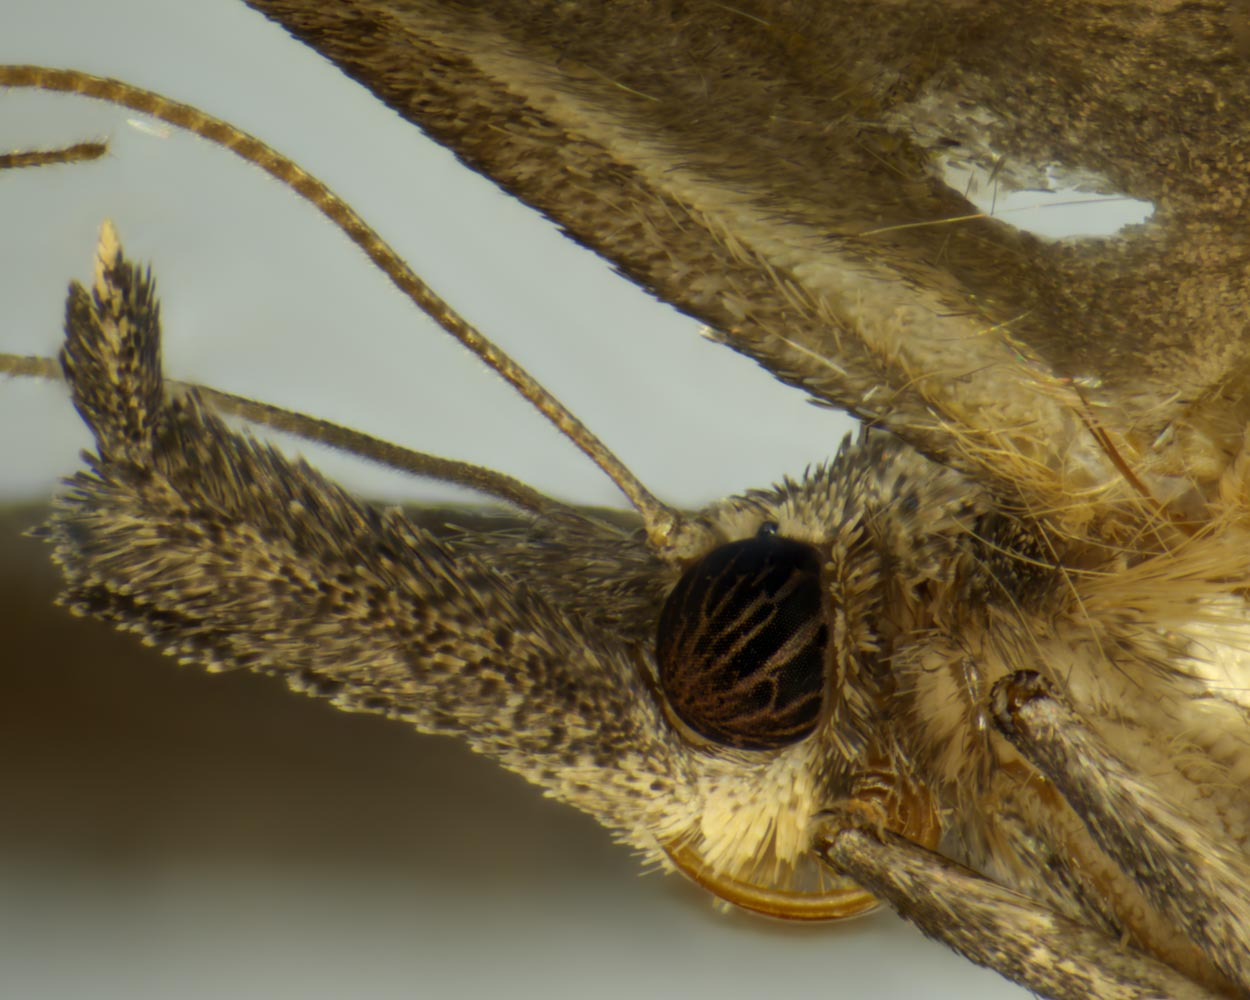
\includegraphics[width=0.9\textwidth]{S202012271446-4} % second figure itself
		\caption{Long, forward facing palps, and oceli above the compound eye of Hypena proboscidalis.}
		\label{fig:S202012271446-4}
	\end{minipage}
\end{figure}

\begin{figure}
	\centering
	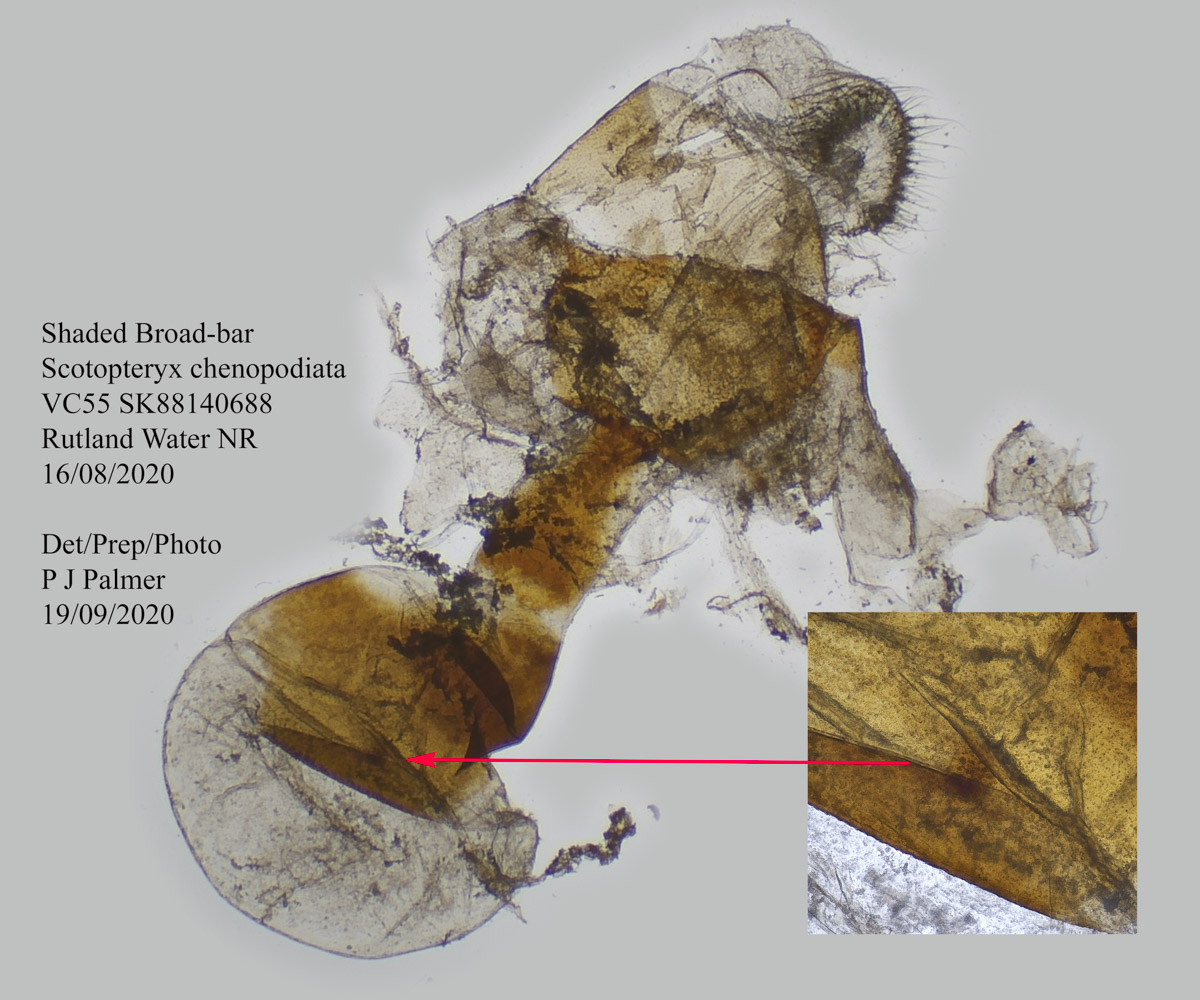
\includegraphics[width=0.7\linewidth]{202009131026PJP-3}
	\caption{Dissection}
	\label{fig:202009131026pjp-3}
\end{figure}


%
%\begin{figure}
%	\centering
%	\includegraphics[width=0.5\linewidth]{images/20201112-1}
%	\caption{Short undamaged palps eliminate Hypena proboscidalis as a candidate taxon.}
%	\label{fig:20201112-1}
%\end{figure}


\bibliography{library}
\end{document}
